\subsection{Tool 2: Android Battery+}
\label{subsec:tool2}

%    This tool is designed both for users and developers and provides
%    real time estimation of screen power consumption.It also provides the user
%    power to regulate device battery life.
%    
%    For example using the tool while travelling user can easily estimate the
%    residual battery life and strike a balance between duration of journey and
%    visual quality by adjusting the brightness.
%     
%    Furthermore,the tool provides the developer the extra ability to fast optimise
%    the screen power by browsing components and fixing priority areas for optimization.

% What is Android Battery ?
Android Battery is a built-in Android utility that helps phone users to
manage the phone battery life by monitoring and exposing the battery drain
per app running on the phone by various components including the CPU,
Wake Lock, Cellular, WiFi, Bluetooth, Sensor, and Camera, but not the
screen. Instead, it simply gives the total screen energy used across
all apps.

% How Android Battery computes screen power ?
Android Battery is implemented in the Battery Stats system service using a simple power model
(power\_profile.xml~\cite{AOSPPowerProfile}) provided by the
manufacturers of various phone components. For screen, the model just
contains the base (at brightness level 0) and the maximum (at brightness level 255) power
consumption. Android Battery then estimates
  per-frame display power as a linear function of the brightness level.
  %  dividing the range of brightness level
%  ({\small \tt  /sys/class/leds/lcd-backlight/brightness}
  % into several bins parameterized with an average screen power for each bin.
  Its screen power estimation is thus frame-content oblivious and can be highly
  inaccurate.
  %  Further, it only reports total screen energy across all apps.}
%   For other components
%   with uses similar mechanism to compute per component energy. Like in
%   CPU there are various power per CPU frequency defined.  The Android
%   Battery will record how much time is spend in various CPU frequency to
%   compute the CPU energy usage.

% Drawback
\if 0
The shortcoming in this approach is though the display power is content 
specific, above power estimation do not take account of this philosophy.
We conducted a simple experiment to validate this. We used android command
{\small \tt dumpsys batterystats --reset} to reset the battery statistics and
dumped subsequent 5 minutes statistics using {\small \tt dumpsys batterystats} for Pixel 2.

We first calculated the power for light and dark mode using our app.
Though we expected a drop of about 66\% display power for dark mode
( as found in Table\ref{fig:powerreductionbrightness}) for 100\% brightness,
we actually observed that for both the modes the statistics (power model) gave us 25.2 mAh.
We repeated this experiment at 50\% brightness and got 12.5 mAh for both light and dark mode.
We extended this experiment to Nexus 6 and Moto Z3 and observed similar results.

This clearly shows that the battery app is not tuned to distinguish between dark and light mode
and can't adequately estimate the dark mode power.
\fi

\paragraph{Android Battery+.}
We enhanced Android Battery by replacing its
simple screen energy calculation
with a new screen energy estimator that uses our new content-based OLED power model
and further accounts the screen energy to individual apps.
We call the new version Android Battery+, or Battery+ for short.
%  The tool we created was combined into the Android Battery to provide the screen
%  display power statistics feature  to the Android Battery.
%  As Battery+ is screen content aware it can distinguish between dark and light mode.
% This tool can easily be extended into the android battery 
% to provide insight to display power component as the percentage
% of total app power for each app.
%  Further, the tool estimates the residual battery life when running the
% app under different screen brightness level.

\if 0
\dcomment{
Like Android Battery, Android Battery+ estimates the screen energy in real
time. It faces two main design challenges.
The first is the computational
overhead in recording every displayed frame and calculating per-frame
display power draw. To control the overhead, we apply pixel sampling
to both screen recording (by modifying the screenrecord command code)
and power calculation (\S\ref{subsec:appl}).
The second challenge is to account screen energy to individual apps.
For this, we modified the Activity manager 
to inform the modified Battery Stats of each app running on the screen
which records the app on-screen
time and implements OLED power and energy calculation per app.
In total, Battery+ is implemented with 1200 LOC in the Android framework and
20 LOC in the Settings app. REMOVED THIS. DESCRIPTION NEXT PARAGRAPH}
\fi


Like Android Battery, Battery+ estimates the screen energy in real
time. 
%  Real time screen energy estimation suffers from the computational
% overhead because of recording every displayed frame and calculating
% per-frame display power draw.
% To control the computational overhead, we have applied pixel sampling to both
% screen recording and power calculation (\S\ref{subsec:appl}).
We first implemented the new screen energy computation module 
by modifying {\small `screenrecord`} command code,
as a 1000 LOC C++ program that runs via the {`adb shell`} interface.
% To invoke this prorgram from Android Battery+, 
%    Further, we incorporated Battery+ into Pixel 2's Android framework for providing
%  an interface via settings app.
% To account screen energy for individual apps, 
We then modified the Activity manager, Battery Stats, and the Settings app
in the Android framework.
In particular, we modified the Activity manager to
inform the modified Battery Stats     of each app running on the screen.
The modified Battery Stats then records the app on-screen time and estimates
the OLED power draw and energy drain per app by calling the screen energy module.
In total, Battery+ is implemented by adding 1200 LOC to
the Android framework and 20 LOC in the Settings app.
We could not implement Battery+ on Moto Z3 as
its framework is not open-sourced.


\if 0
The mobile display has a large number of pixels.For example Nexus 6
has 3.7 Mpx, Pixel 2 has 2.1 Mpx and Moto Z3 has 2.3 Mpx.
Capturing the entire screen and estimating screen power considering all
the pixels increases the computations tremendously.
For this we used pixel sampling to estimate the current resulting in low
overhead.

In the current state the android battery can only estimate power at the device
level which lacks ability to estimate  app screen power estimation.
Hence,we  implemented a mechanism to calculate, record and display per
app time spend on the screen and their average screen power consumption.

We experimentally observed that estimation of power using entire
screen pixel is not required i.e.  sampling down to 1\% of the total
pixel can provide adequate estimation accuracy.  The accuracy is given
in Figure~\ref{fig:smapling_error}.  We can see that the average error
of estimation using this approach is less than 1\%.  The overhead
requirement observed with different sampling ratios is provided in
Figure~\ref{fig:tool2_screenshot} . We can see that with 1\% of pixel
sampling the average time taken for predicting power per frame is
below 16 ms for all the three phones. For Pixel 2 and Moto Z3 it takes
about 4 mS and for Nexus 6 it takes about 13 mS. For Nexus
6,corresponding average reduction in CPU overhead is from 20\% to 5\%.


% We modified it to fetch the frame from the frame buffer at 
%  We used the captured frame to estimate the display current using the P-LMMR.
%  We packaged all the above in an user-friendly  Android app.
%  The display current estimation is drawn in the foreground over other apps in a small box.
%  The screen shot of the app is given in Figure\ref{fig:tool2_screenshot}
\paragraph{Implementation.}
We implemented Battery+ on AOSP Nougut 7 for Nexus 6.
We modified the screenrecond command code base to implement
frame recording at 1\% pixel sampling.
% We keep the track on the screen energy consumed during the device run.
Battery+ queries the screen energy at the time when the app comes on
the top of and when it leaves the screen.
The different of the screen energy consumed is taken as the screen energy
consumed by the app.
The Battery+ design is shown in Figure~\ref{fig:tool2_arch}.
The Activity Manger takes care of all the running apps.
We modified the Activity Manager to notify the Battery Stats mechanism of
the app displayed on the screen.
In the battery stats we call the our tool (shown as Display Current)
to get the screen energy during the duration of the total run of the app.
When the android settings app for battery is called the screen information is
passed onto the Battery Stats Helper which in turn communicates to the android settings app.
We modified the system app Settings and added five components per app i.e.
the total screen time ,the average screen power, estimated time the app can run on battery
for 30\%, 50\% and 100\% brightness levels.


\fi

\if 0
\begin{figure}[h]
	\begin{subfigure}[]{0.4\columnwidth}
		\includegraphics[width=\textwidth]{./figure/12001_current.png}
		\caption{The yellow box shows the display current in a floating window
			for the real time screen current. (on Pixel 2)}
	\end{subfigure}
	\hfill
	\begin{subfigure}[]{0.4\columnwidth}
		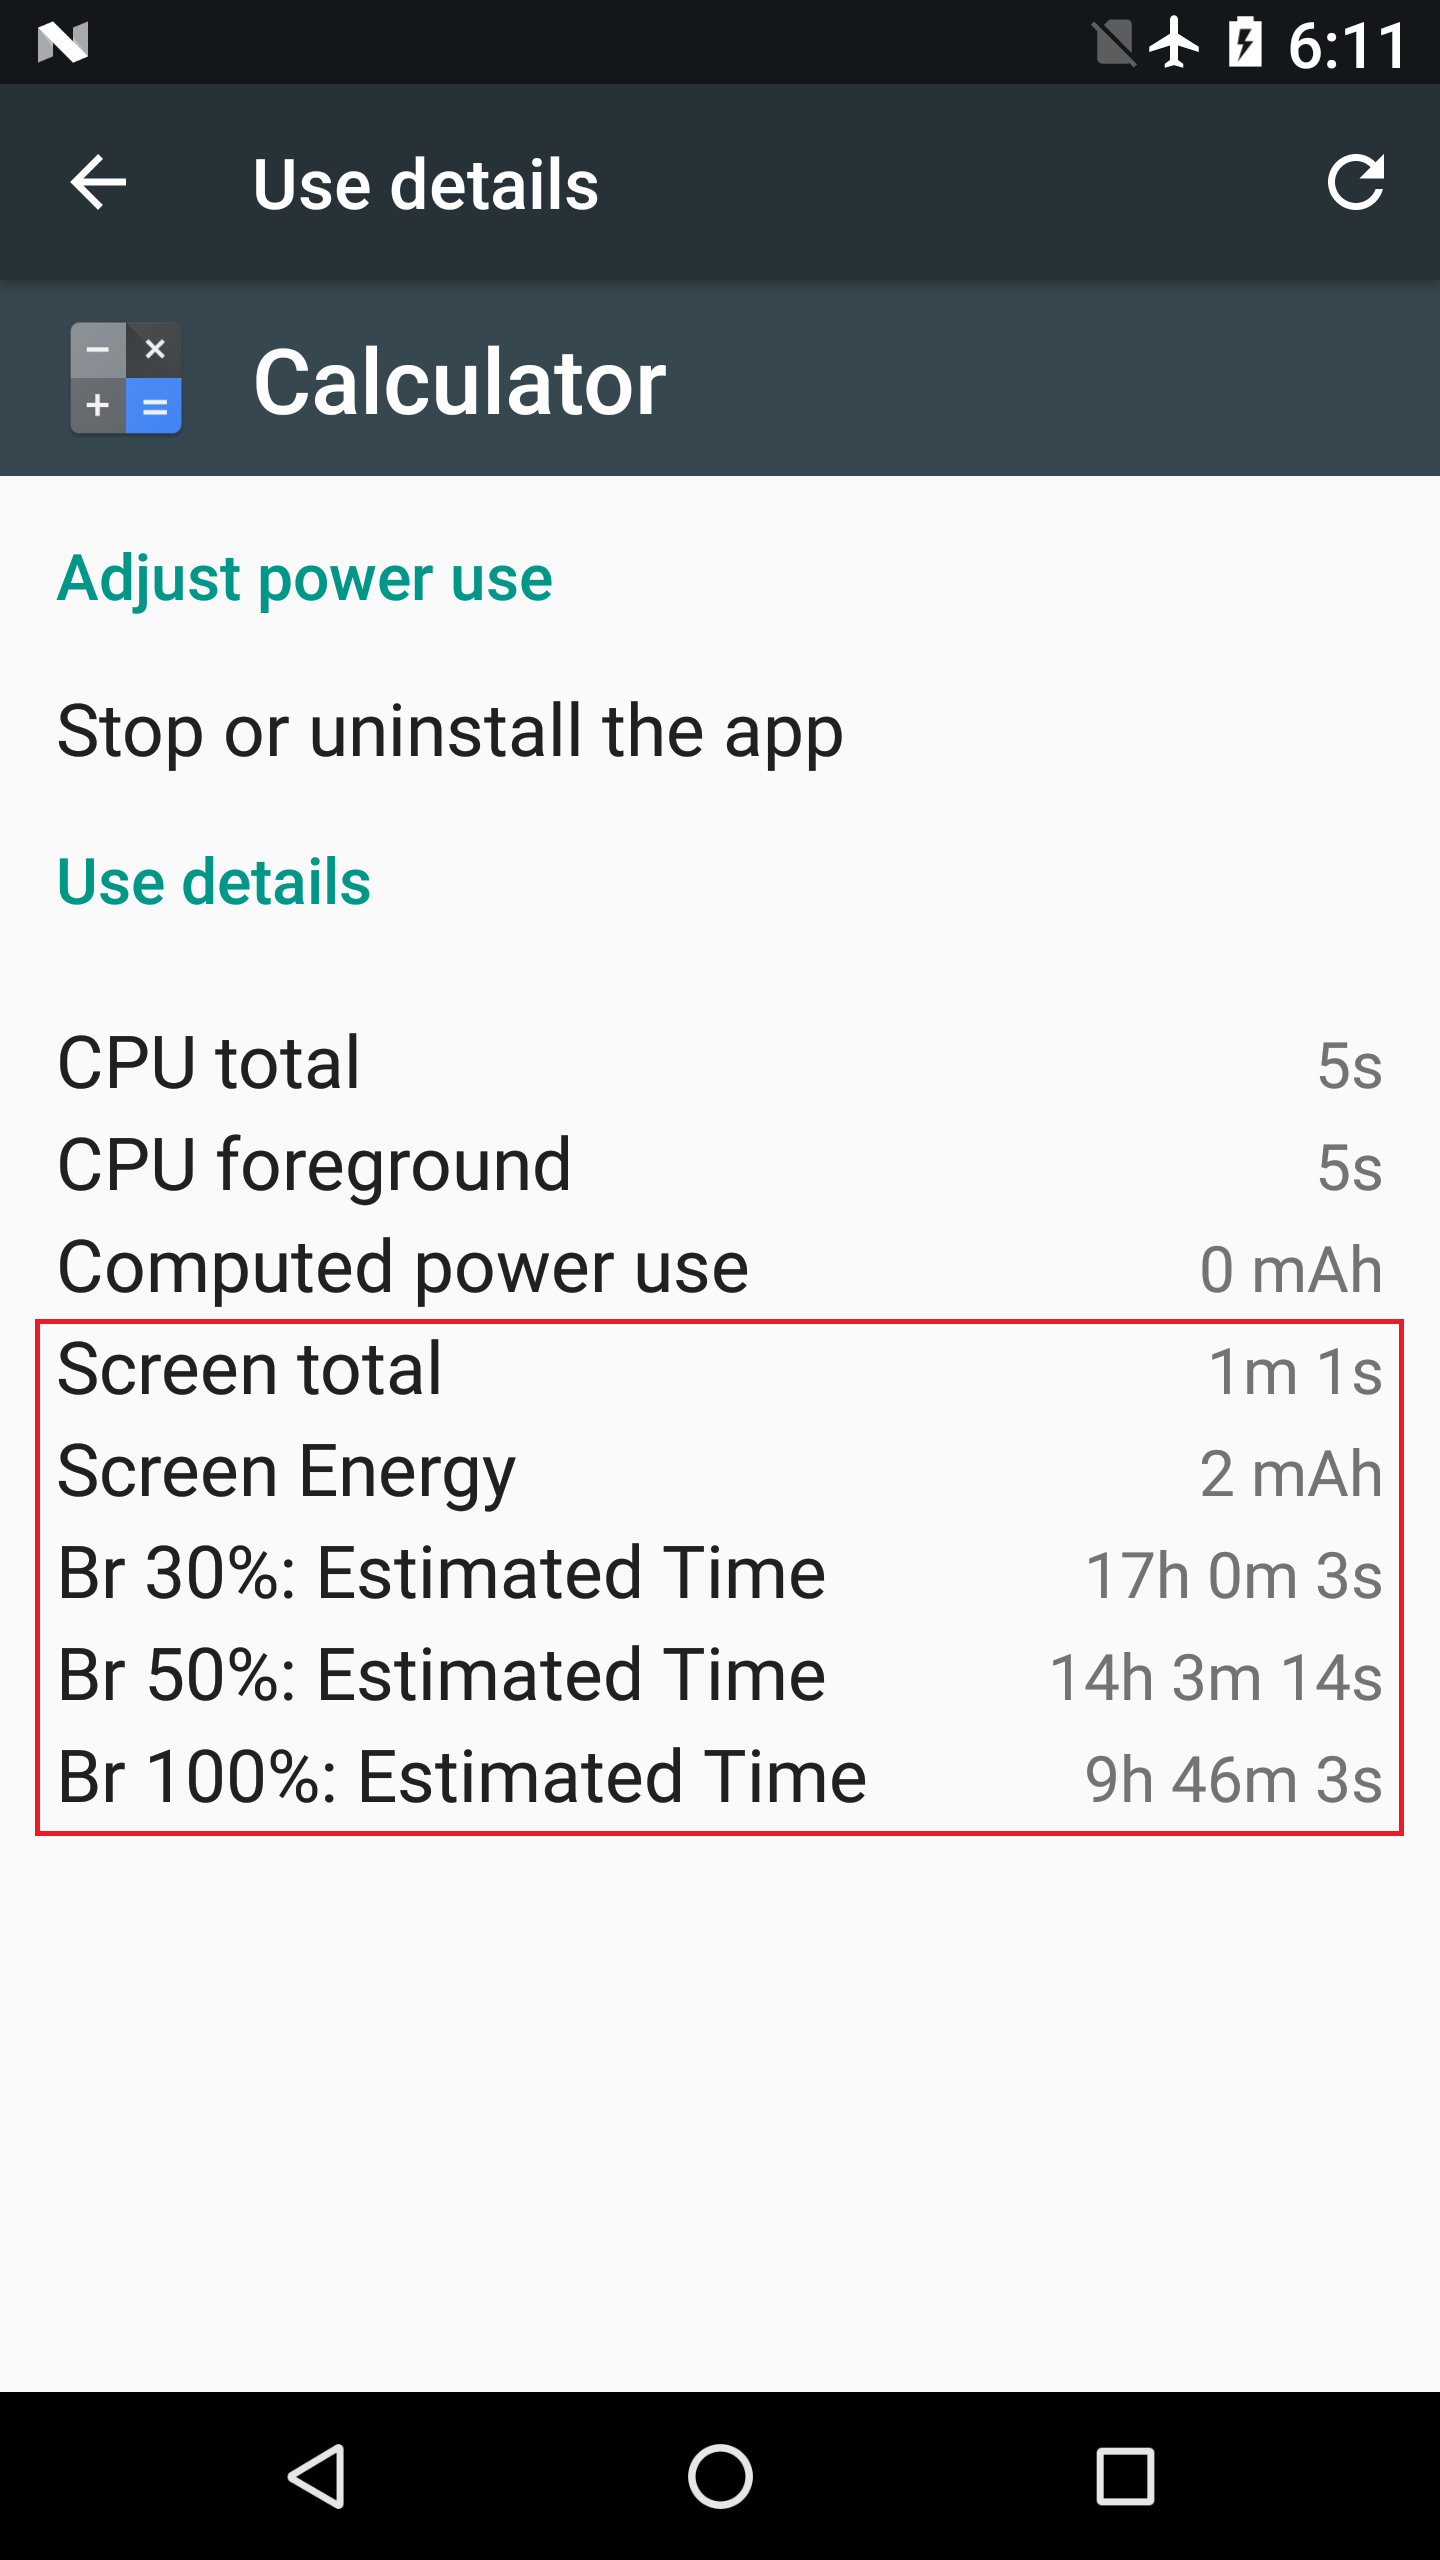
\includegraphics[width=\textwidth]{./figure/513_abat_plus_screenshot.png}
		\caption{Battery+: The entries in the red box is
			added by us. (on Nexus 6)}
	\end{subfigure}
        \vspace{-0.1in}
	\caption{Screen Shots}
	\label{fig:tool2_screenshot}
\end{figure}
\fi

\if 0
\begin{figure}[h]
	\begin{subfigure}[]{\columnwidth}
		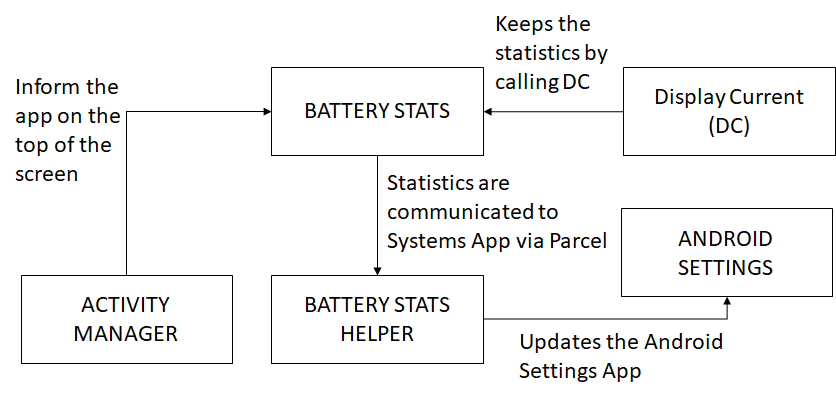
\includegraphics[width=\columnwidth]{./figure/512_arch.png}
	\end{subfigure}
        \vspace{-0.1in}
	\caption{Design Architecture}
	\label{fig:tool2_arch}
\end{figure}

\begin{figure}[h]
	\begin{subfigure}[]{\columnwidth}
		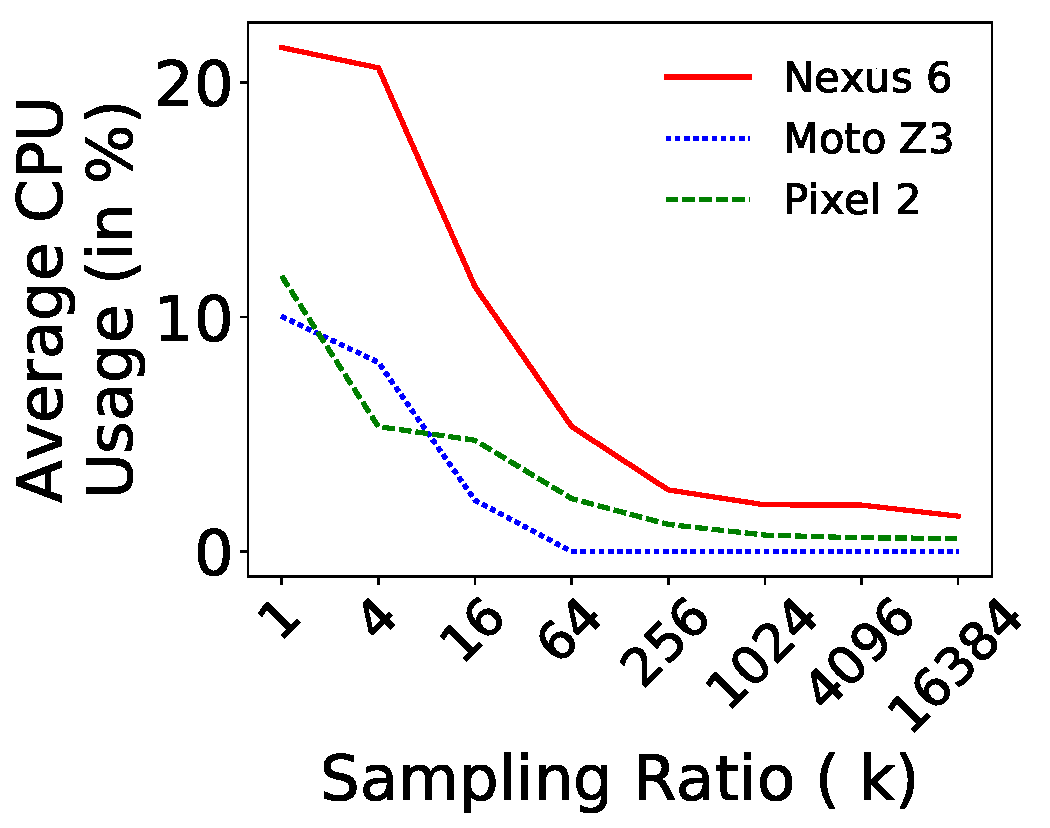
\includegraphics[width=0.48\columnwidth]{./figure/511c_All_overhead.pdf}
 		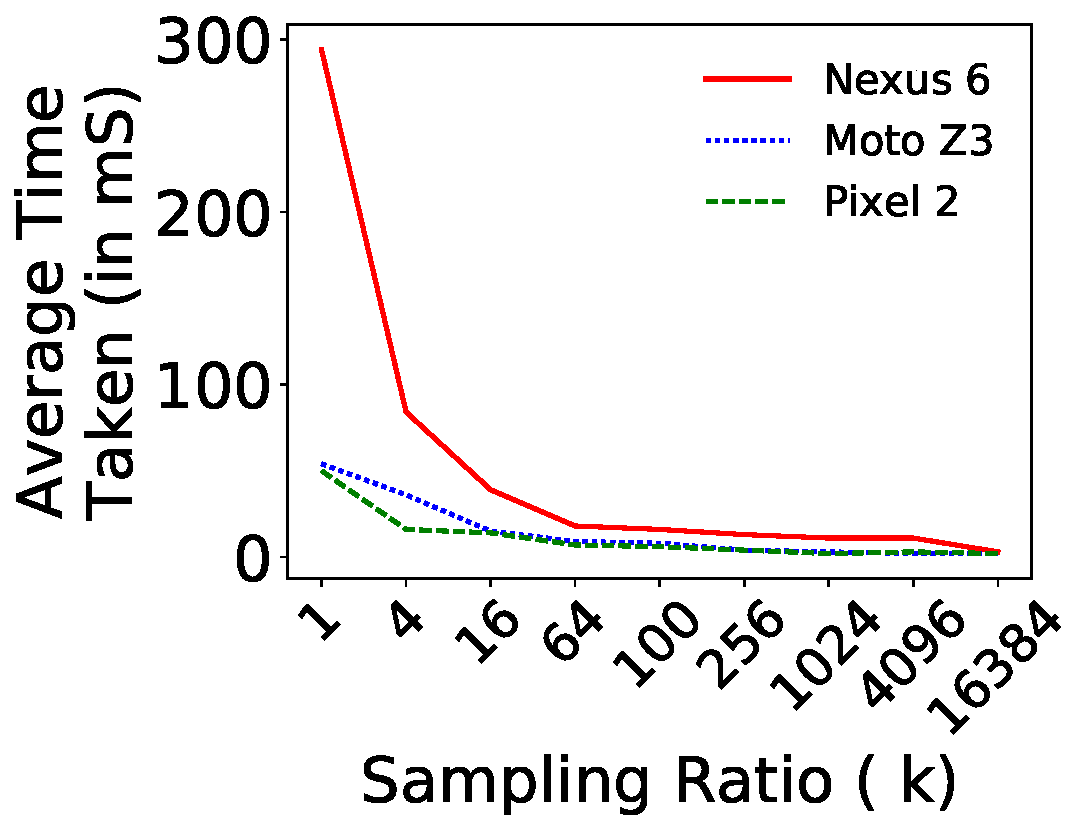
\includegraphics[width=0.48\columnwidth]{./figure/511b_All_time.pdf}
	\end{subfigure}
        \vspace{-0.1in}
	\caption{Overhead of Tool 2 at various sampling ratio}
	\label{fig:tool2_overhead}
\end{figure}
\fi


% \begin{figure}[h]
% \begin{minipage}{\columnwidth}
% 	\begin{subfigure}[]{0.35\columnwidth}
% 		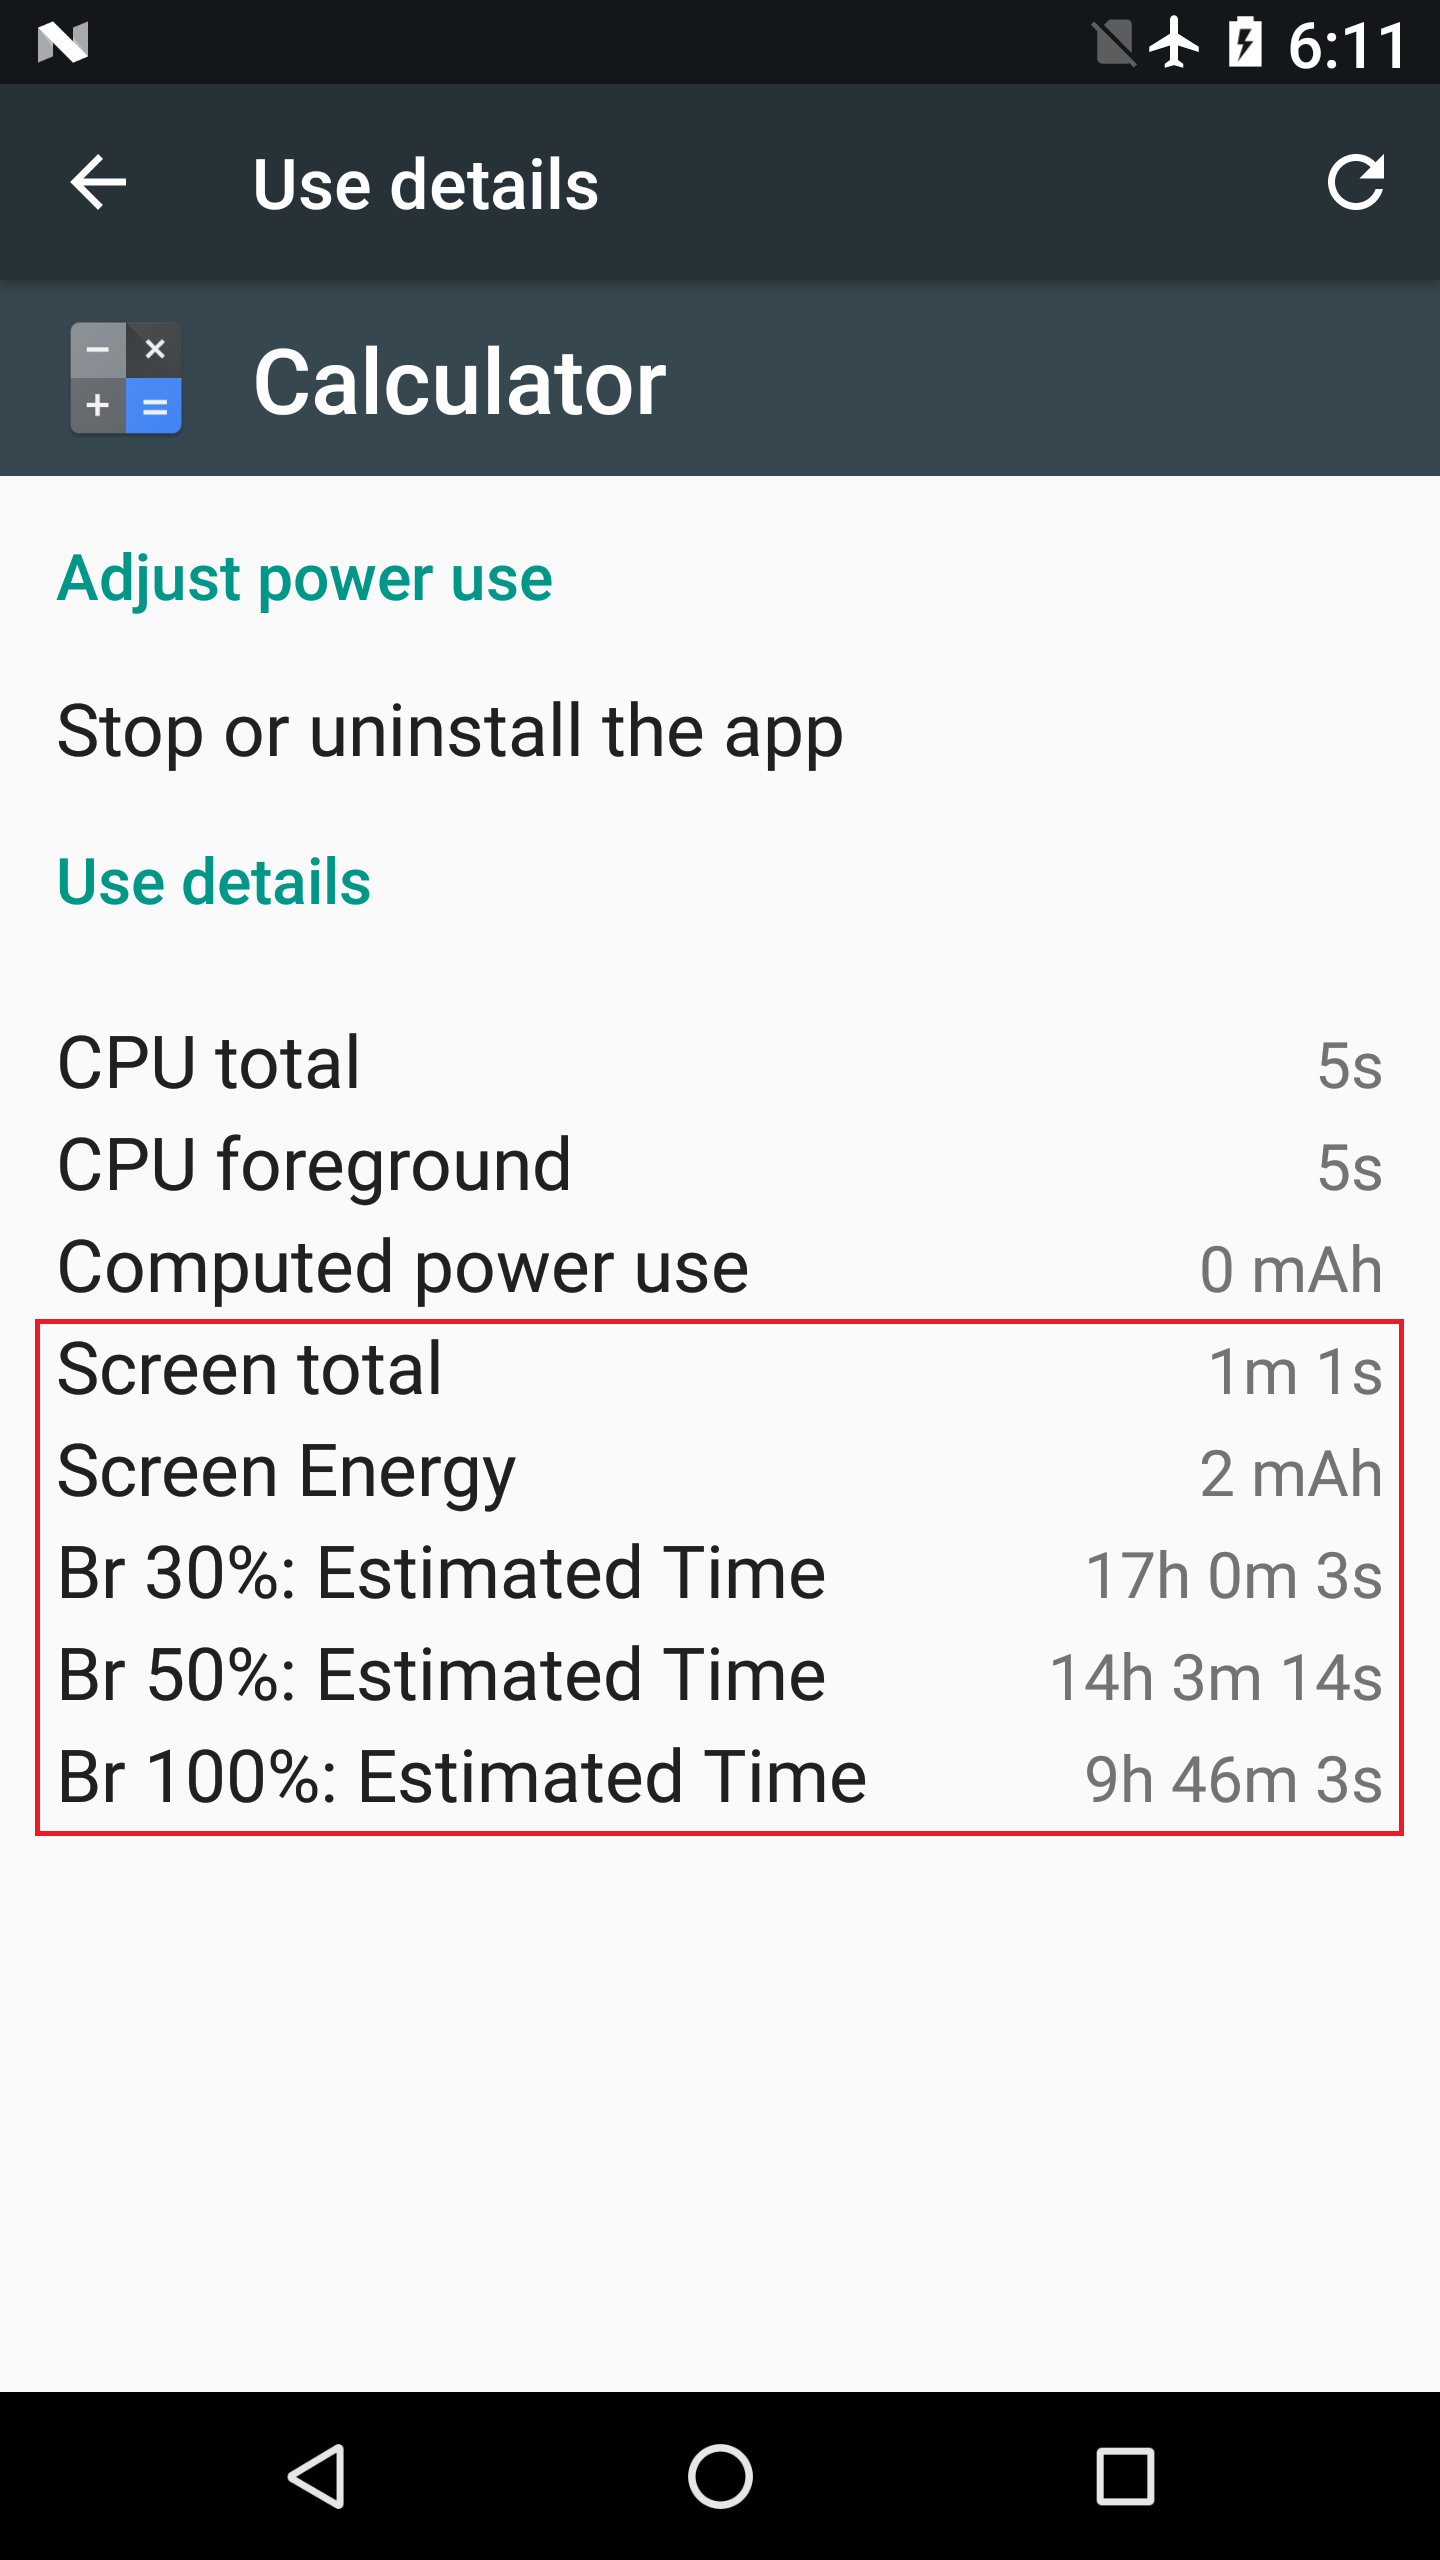
\includegraphics[width=\textwidth]{./figure/513_abat_plus_screenshot.png}
% 		\caption{The entries in the red box is added by us.}
% 	\end{subfigure}
% 	\hfill
% 	\begin{subfigure}[]{0.60\columnwidth}
% 		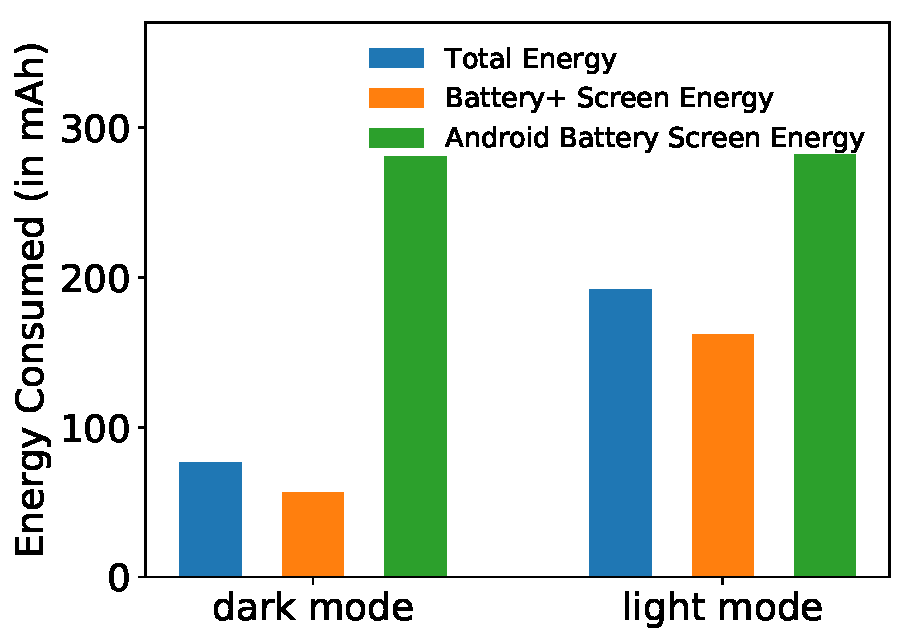
\includegraphics[width=\textwidth]{./figure/513_battery_compare.pdf}
% 		\caption{Comparing with Android Battery for Google Calculator App.}
% 	\end{subfigure}
%         \vspace{-0.1in}
% 	\caption{Battery+: Screenshot of Android Settings and comparison with Android Battery on Nexus 6}
% 	\label{fig:tool2_screenshot}
% \end{minipage}
% \end{figure}

\begin{figure}[tp]
\begin{minipage}{0.35\columnwidth}
	\begin{subfigure}[]{\textwidth}
		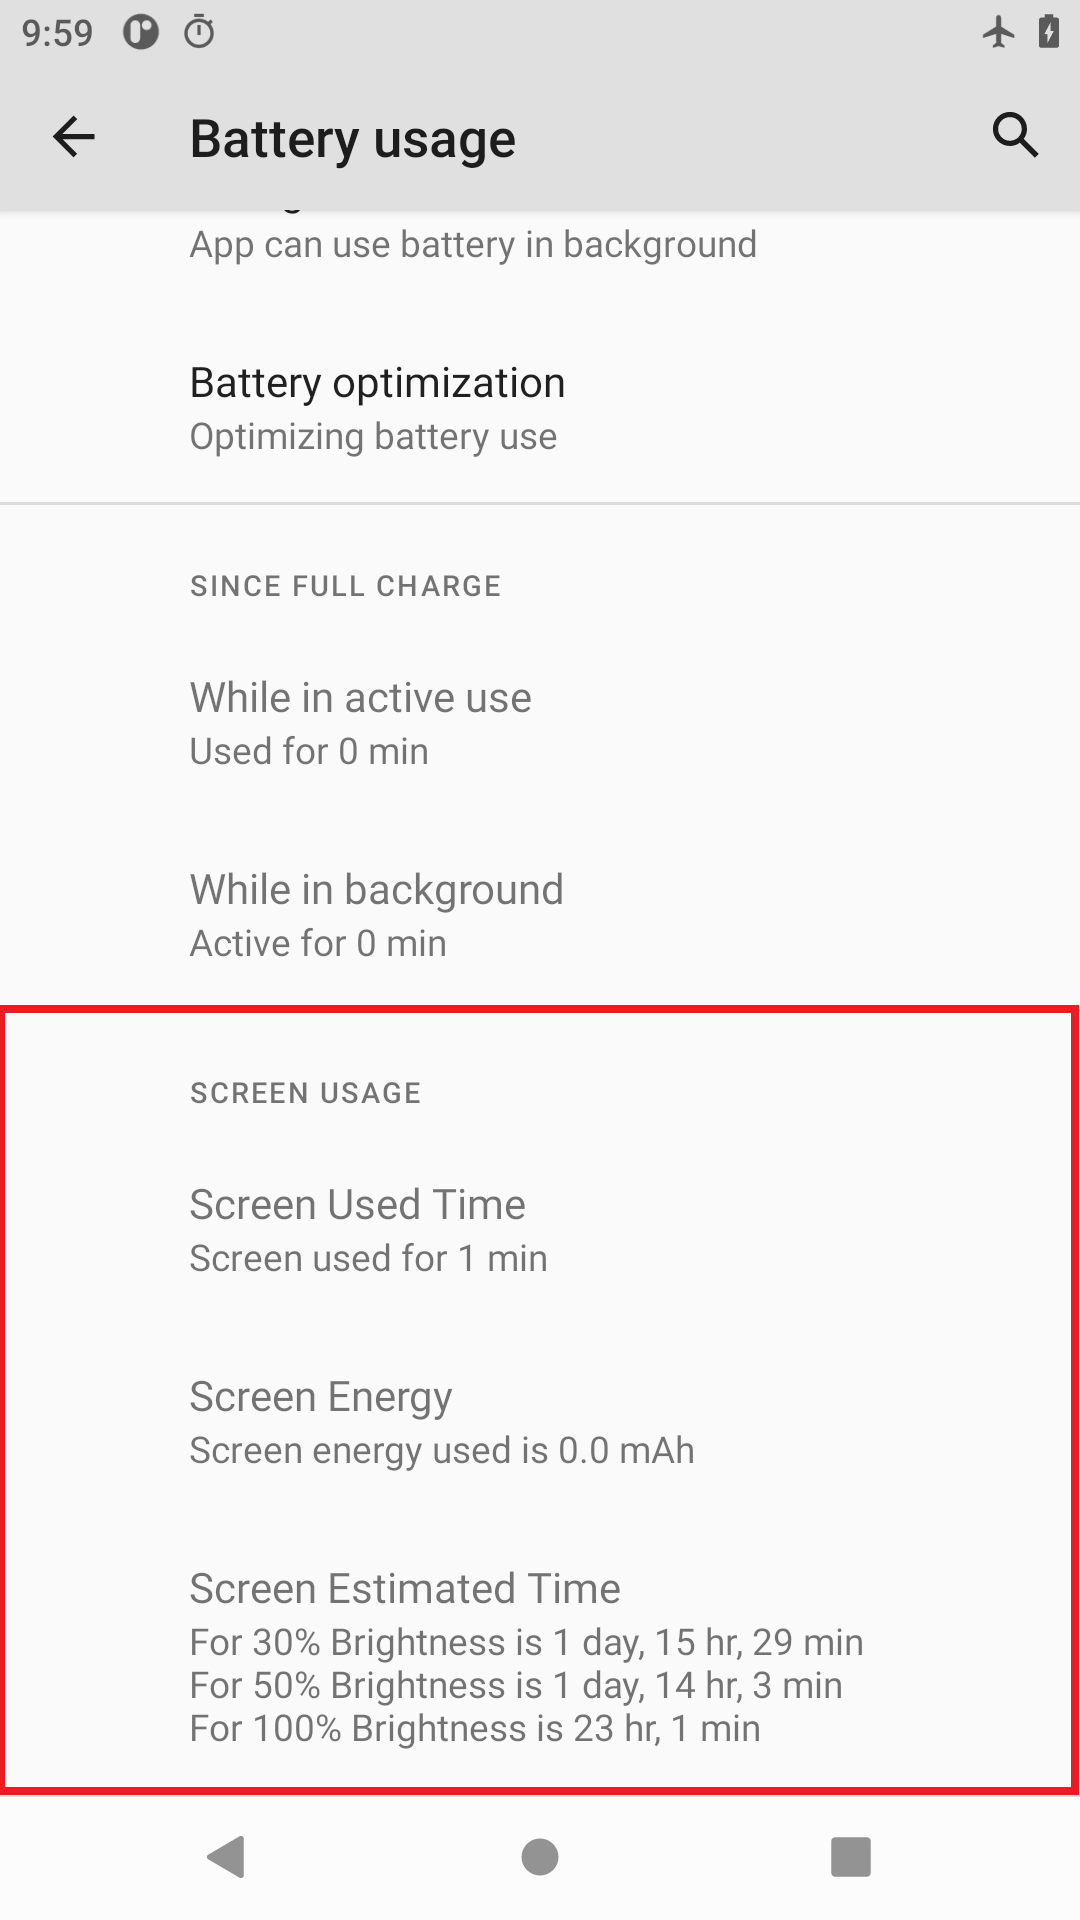
\includegraphics[width=\textwidth]{figure/001_Battery_app_screencap.png}
	\end{subfigure}
        \vspace{-0.1in}
	\caption{Screenshot of Android Settings.
          The red box contains new entries added in Battery+.}
        \vspace{-0.2in}
	\label{fig:tool2_screenshot}
\end{minipage}
\hfill
\begin{minipage}{0.60\columnwidth}
	\begin{subfigure}[]{\textwidth}
		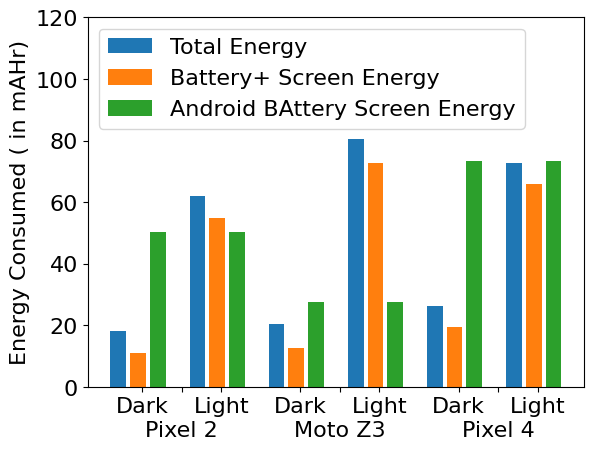
\includegraphics[width=\textwidth]{figure/battery+_screen_energy_compare.png}
	\end{subfigure}
        \vspace{-0.1in}
	\caption{Comparing Battery+ and Android Battery screen energy for the Google Calculator app.}
	\label{fig:tool2_battery_compare}
        \vspace{-0.2in}
\end{minipage}
\end{figure}

\paragraph{Evaluation.}
We first measured the overhead of Battery+'s
screen energy module while running the camera app on
screen for 10 minutes.  As reported in \S\ref{subsec:appl}, at a pixel
sampling ratio of 100, the latency of per frame recording is
4ms, 3ms, and 2ms on Pixel 2, Moto Z3, and Pixel 4, respectively, while incurring less than
1\% 
additional prediction error.  We then isolated the modified Battery Stats
process and measured its CPU usage; the average CPU utilization is
only 1.12\%, 0.92\%, and 0.59\% for the three phones, respectively.

Next, we compared the screen energy accuracy by 
Battery+ and Android Battery.
We ran the calculator app for 10 minutes twice, first in light mode and then in
dark mode, under full screen brightness.
% Battery+ captures the screen and total energy consumed. 
Figure~\ref{fig:tool2_screenshot} shows a screenshot of
Battery+ on Pixel 2, where it shows the total screen time and screen energy
for the app.
Figure~\ref{fig:tool2_battery_compare} plots the
total phone energy drain based on the battery level drop (same by  both tools)
and the screen energy estimated by Android Battery and Battery+,
under dark and light modes, respectively.
We observe that
(1) Android Battery is oblivious to screen content and incorrectly reports
the same screen energy under the two modes;
in particular, it over-estimates the  OLED display power draw in dark mode
to be 4.62$\times$ (50.39 mAh vs.\ 10.91 mAh), 
2.15$\times$ (27.59 mAh vs.\ 12.82 mAh), 
3.75$\times$ (73.46 mAh vs.\ 19.57 mAh)
higher than the total phone power draw, on the three phones, respectively.
(2) In contrast, Battery+ correctly estimates the impact of the dark mode,
as shown by the same non-OLED power draw, \ie the difference 
between the total phone power draw and the OLED display power draw,
under light and dark modes.
\if 0
(2) Android Battery overestimates screen energy vs. Battery+ is
% by 5.0$\times$ (281 mAh vs. 56.2 mAh under Battery+) under dark mode
% and 1.7$\times$ (282 mAh vs. 162 mAh under Battery+) under light mode,
% which are even higher than the total app energy!
151 mAh vs. 29 mAh for dark and 163 mAh for light mode for Pixel 2,
83 mAh vs. 38 mAh for dark and 217 mAh for light mode for Moto Z3, and
222 mAh vs. 58 mAh for dark and 196 mAh for light mode for Pixel 4.
Which is even higher than the total app energy for dark mode!
\fi

\if 0
We did an overhead analysis for the tool2 which is shown in Figure~\ref{fig:tool2_overhead}.
We observed that time taken for 1\% sampling is less than 16 ms for all the phones
as noted earlier and this  implies that tool2 can work with display refresh rate up to 60 FPS.

We conclude from the above that the we can gather the statics at
60 FPS with CPU overhead of about 5\% and less.

Next, we compared Battery+ with Android Battery in terms of accuracy.
We ran the calculator app for 30 mins twice, first in light mode and then in
dark mode. Battery+ captures the screen and total energy
consumed. 
Figure~\ref{fig:tool2_battery_compare} shows a screenshot of
Battery+ on Nexus 6, where it shows the total screen time and screen energy
for the app.
Figure~\ref{??} plots the
total phone energy drain based on battery level drop;
and the screen energy estimated by Android Battery and Battery+,
under dark and light modes respectively.
We observe that
(1) Android Battery is oblivious to screen content and hence
dark mode and reports the same screen energy under the two modes;
(2) Android Battery overestimates screen energy
by ??$\times$ (??mAh vs ??mAh under Battery+) under dark mode
and ??$\times$ (??mAh vs ??mAh under Battery+) under light mode,
which are even higher the total app energy.
\fi

\if 0
estimates total power consumed of about 23.4 mAh in dark and 64.2
mAh in light mode.  We can also see from the figure that the screen
power estimated by android battery is 94.4 mAh i.e same for both
light and dark mode and this exceeds the total power consumed
indicating that these estimations are not accurate.  In addition to
total power the screen power estimated by the Battery+ is 15.3 mAh
for dark and 51.0 mAh for light mode.  From the we can approximate
the non-screen component which is 8.1 mAh for dark and 13.2 mAh for
light mode.  
\fi

\if 0
\begin{figure}[h]
	\begin{subfigure}[]{\columnwidth}
		\centering
		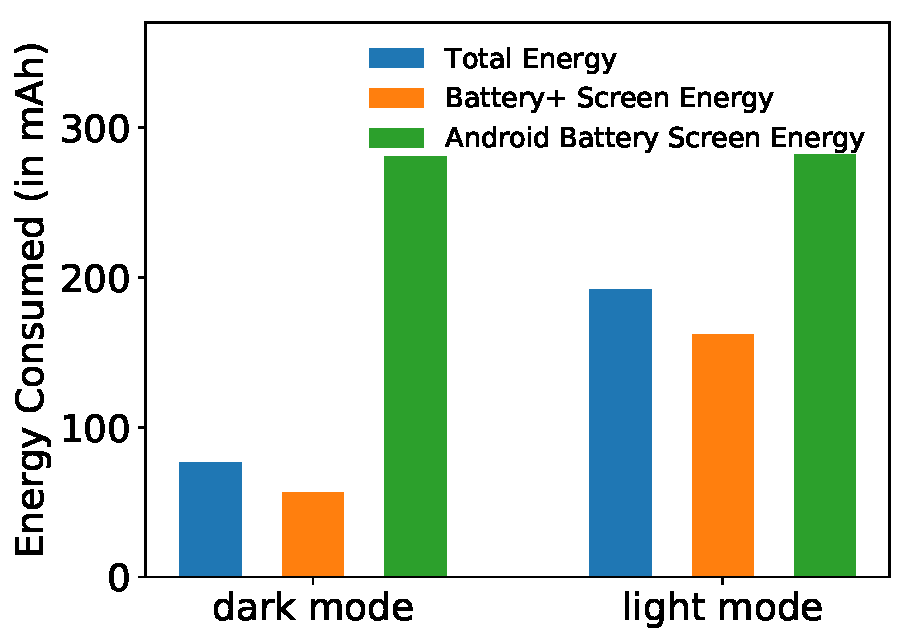
\includegraphics[width=0.8\columnwidth]{./figure/513_battery_compare.pdf}
	\end{subfigure}
        \vspace{-0.1in}
	\caption{Comparing Android Battery with Battery+ for Google Calculator App.
\comment{make y-ais go up t 300 or 350 so you an enlarge the legend???}}
	\label{fig:tool2_battery_compare}
\end{figure}
\fi
% We recorded various popular apps (apps are listed in ~\ref{tab:experiments}).
% Using these app runs we  observed that the
% Display current estimation is off by on average of 3\%-10\% from measured current.
% 
% The app is also capable to handle brightness corrections.
% We use this app to evaluate our case study on activities.
% Table~\ref{tab:Dark_vs_light_popular_google_apps} shows all the results.
% 
% The overhead of the tool in plotted in Figure~\ref{fig:tool2_screenshot} with various frame rate
% And sampling ratio of the screen.

%%%%%%%%%%%%%%%%%%%%%%%%%%%%%%%%%%%%%%%%%%%%%%%%%%%%%%%%%%%%%%%%%%%%%%%%%%%
\if 0
\subsection{Tool 3: Fast Modeling}

\subsubsection{Objective:}
We observed that Pixel2 and Moto Z3 has power sensor with a sampling rate of approximately
1.4 second .Using this sampling rate the static model generation will take
more 12 hrs with 4096 piecewise model and more than 2 hrs with 512 model.
The main problem is we need to take care of the experiment very
precisely during the long test duration, like the external environmental conditions like temperature.

We observed for the UI of apps (listed in ~\ref{tab:experiments}), the histogram has very distinct and
has few peaks. This happens because the activities are synthetically colored.
The spread in the histogram happens in case there is a
dynamic object which may have continuous textures. When designing
the UI, the developer will not consider these objects as these are updated
at the runtime.

This is also true that designer must evaluate their app on various devices
before they release the app. So, modeling and optimizing app in various devices is very time
consuming process given that a UI design consists of a small proportion of colors.

\subsubsection{Design Challenges:}
We need to detect the components on the screen so as to determine
the dynamic components. We do this by using the Per Component Analyzer.
We have to generate the histogram and observe the peaks.(??)

There might be some continuous components in the activity which may not contribute
to more than 1\% like the shadowing of the text. For this we switch to the linear model.
As we have seen earlier we estimate the red, blue and green curve in linear RGB,
by only knowing the lowest and highest intensity current. So in total for this we
require 4 (as the lowest intensity in all red, green and blue is black) images to evaluate the current.
The error in linear model is high but it will be a small fraction of the screen and
this error with respect to total display current will be very small.

\subsubsection{How to Solve?:}
We generate the histogram of the entire screen. We find all peaks which have
a contribution to the screen area more than 1\% of the screen area.

\subsubsection{Implementation:}
We created an Android app for this purpose.
We brought the Android screenrecord and screencap command code. We fetch
the screen and generate an histogram.
We identify the peaks. We go into a app training mode where the model is evaluated
by displaying monochromatic images on the screen. Each of the image is shown for 5 to 10
seconds.
If the peaks do not cover 99\% of the screen , we also calibrate 4 more images i.e.
black, read, green and blue at full intensity for linear model.

\subsubsection{Evaluation:}
\fi

